% mainfile:main.tex

\chapter{Tab Groups}

\section{Analysis and design}

gedit is currently using a multiple document interface, called \emph{MDI}. By the use of tabs it provides a way to visualize several documents in a single window. With the current interface gedit has the problem that it can not show different documents at the same time, the only way right now, it is to open two gedit windows and resize them to fit the screen. This is very tedious and uncomfortable for the user.

\subsection{Questions}

Knowing this problem, when brainstorming in the different possibilities about implementing this, the next questions showed up:
\begin{enumerate}
  \item How do we show the extra document to the user? Different tab groups or inside a tab?
  \item How do we want to allow the split? Vertically, Horizontally or allow both?
  \item How many side documents should we allow?
\end{enumerate}

\subsection{Do not reinvent the wheel}

When analyzing a problem, the gedit team has something very clear, check what are doing the other competitors, analyze their ideas and decide which one could fit better our requisites. Before answering the questions the programs below have been checked:

\subsubsection{Netbeans}

In the figure \ref{fig:NetbeansScreenshot} it can be shown that this program allows to have several tab groups\footnote{By tab groups we refer to the ability of grouping tabs in different groups that can be viewed at the same time in a window} and group them either horizontally and vertically. This is due to the fact that netbeans uses a docking system which allows it to place the tabs whichever the user prefer. In GTK+ there is not any widget or way to provide this ability, there is another library called \emph{GDL} that provides this and it is used by programs like anjuta, but it has the problem that it is not very well maintained and it would produce problems in the future.

\subsubsection{Kate}

In relation to kate as shown in the figure \ref{fig:KateScreenshot}, we can see that it does not have proper tabs as in gedit, it has a side pane showing the documents and it allows to open the documents either vertically or horizontally. This solution escapes from the sense of gedit and in our opinion can make things not very discoverable for the end-up user.

\subsubsection{Notepad++}

In the figure \ref{fig:NotepadScreenshot} we can see that it has a similar interface to the one in gedit. It allows to create only one more tab group and it only makes an horizontally split.

\newpage
\addfigure[scale=0.29]{./images/netbeans}{Netbeans screenshot}{fig:NetbeansScreenshot}

\addfigure[scale=0.29]{./images/kate}{Kate screenshot}{fig:KateScreenshot}

\newpage
\addfigure{./images/notepad}{Notepad screenshot}{fig:NotepadScreenshot}

\subsection{Answering to the questions}

\begin{enumerate}
  \item Tab groups fit better the current gedit design and it will make it easier to use for the user and easier to implement.
  \item Horizontal split makes sense for visualizing documents side by side. Vertical split makes more sense if you are editing the same document in different parts of it. I.e having splitted the document to edit and show several parts of it.
  \item It was decided to allow n splits. It is up to the user to decide how many splits he wants. If at some point is needed to put some restriction, it would be easier to make it.
\end{enumerate}

\newpage
\subsection{Prototyping}

In the figure \ref{fig:TabGroupsProto1} it can be shown a prototype made with glade in relation how it would look and what kind of widgets will be used. In the figure \ref{fig:TabGroupsProto2} it has been made a prototype also that helped to answer the questions above, showing the vertical split. Apart from the visual design some points must be taken into account:
\begin{enumerate}
  \item By default a gedit window has a single tab group (current behavior).
  \item The same document can NOT appear in different tab groups or different tabs.
\end{enumerate}

\begin{figure}[H]
  \begin{minipage}[b]{0.5\linewidth}
    \centering
    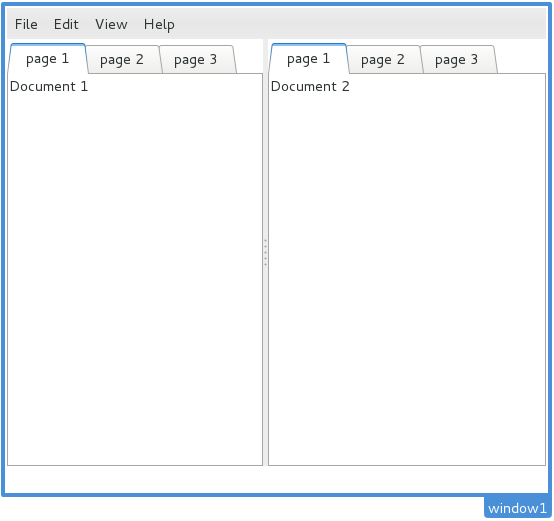
\includegraphics[scale=0.40]{./images/tab-groups-proto-1}
    \caption{Tab groups prototype 1}\label{fig:TabGroupsProto1}
  \end{minipage}
  \hspace{0.5cm}
  \begin{minipage}[b]{0.5\linewidth}
    \centering
    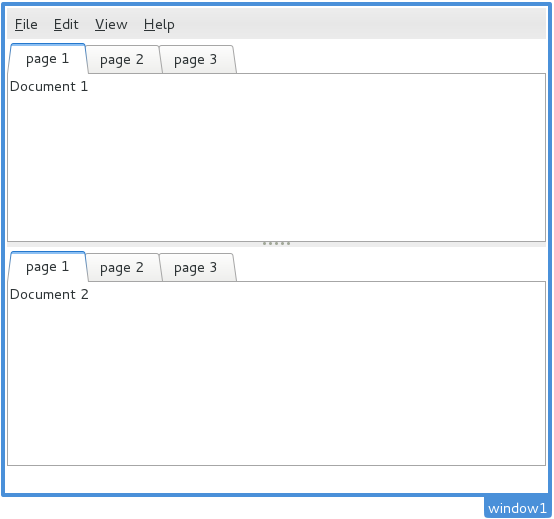
\includegraphics[scale=0.40]{./images/tab-groups-proto-2}
    \caption{Tab groups prototype 2}\label{fig:TabGroupsProto2}
  \end{minipage}
\end{figure}

\newpage
\subsection{Class diagram modification}

\addfigure[scale=0.45]{./images/tab-groups-diagram}{Tab groups diagram}{fig:TabGroupDiagram}

As it can be visualized in the figure \ref{fig:TabGroupDiagram} a new class has been introduced, \emph{GeditMultiNotebook}. This class will take care of create and remove GeditNotebooks, proxying the signals emittion for page-added, page-removed and switch-page and it will be kept as an implementation detail where the user will not have direct access to its API.

\newpage
\subsection{GeditMultiNotebook}

This class works as a proxy to \emph{GeditNotebook}, most of the API and signals are the same, here will be explained the different methods and signals.

\subsubsection{Signals}

\begin{table}[H]
  \begin{center}
    \begin{tabularx}{\textwidth}{|l|X|}
      \firsthline
      \textbf{Signal name:} & \textbf{Explanation:} \\
      \hline
      \textit{notebook\_added} & emitted when a new notebook has been added. \\
      \hline
      \textit{notebook\_removed} & emitted when a notebook is removed. \\
      \hline
      \textit{tab\_added} & proxy signal for page\_added from GtkNotebook. \\
      \hline
      \textit{tab\_removed} & proxy signal for page\_removed from GtkNotebook. \\
      \hline
      \textit{switch\_tab} & proxy signal for switch\_page from GtkNotebook. \\
      \hline
      \textit{tab\_close\_request} & proxy signal for tab\_close\_request from GeditNotebook. \\
      \hline
      \textit{page\_reordered} & proxy signal for page\_reordered from GtkNotebook. \\
      \hline
      \textit{show\_popup\_menu} & emitted when the right button of the mouse is clicked in the notebook. \\
      \lasthline
    \end{tabularx}
    \caption{Tab groups signals explanation}
  \end{center}
\end{table}

\begin{table}[H]
  \begin{center}
    \begin{tabularx}{\textwidth}{|l|X|}
      \firsthline
      \textbf{Method name:} & \textbf{Explanation:} \\
      \hline
      \textit{get\_active\_notebook} & Gets the active notebook \\
      \hline
      \textit{get\_n\_notebooks} & Gets the number of notebooks, at least there will be one \\
      \hline
      \textit{get\_nth\_notebook} & Gets the n notebook of the list \\
      \hline
      \textit{get\_notebook\_num} & Given a notebook get the number in the list \\
      \hline
      \textit{get\_n\_tabs} & Returns the number of tabs in all the notebooks \\
      \hline
      \textit{get\_page\_num} & Finds the index of the page which contains the given tab \\
      \hline
      \textit{get\_active\_tab} & Gets the active tab \\
      \hline
      \textit{set\_active\_tab} & Sets the active tab \\
      \textit{set\_current\_page} & Sets the active tab in relation to the total pages \\
      \hline
      \textit{get\_all\_tabs} & Gets all the tabs \\
      \hline
      \textit{close\_tabs} & Closes a list of tabs \\
      \hline
      \textit{close\_all\_tabs} & Closes all tabs \\
      \lasthline
    \end{tabularx}
  \end{center}
\end{table}

\newpage
\begin{table}[H]
  \begin{center}
    \begin{tabularx}{\textwidth}{|l|X|}
      \firsthline
      \textit{add\_new\_notebook} & Adds a new notebook \\
      \hline
      \textit{remove\_active\_notebook} & Removes the active notebook \\
      \hline
      \textit{previous\_notebook} & Focuses the previous notebook \\
      \hline
      \textit{next\_notebook} & Focuses the next notebook \\
      \lasthline
    \end{tabularx}
    \caption{Tab groups methods explanation}
  \end{center}
\end{table}

\section{Implementation}

When this was implemented there were two things depending directly on GeditNotebook. \emph{GeditDocumentsPanel} (see figure \ref{fig:GeditDocumentsPanel1}) which shows in the side panel the currently opened documents and allows to manage them, and the \emph{Documents menu} which showed the documents and set shortcuts\footnote{A shortcut is a set of keys which allows to invoke a specific action.} to them, to switch easily between the documents pressing Control+\#. These two features were disabled in order to be able to start the implementation.

\addfigure[scale=0.60]{./images/gedit-documents-panel1}{Documents panel}{fig:GeditDocumentsPanel1}

In order to implement it, an intensive use of \emph{GtkHPaneds}\footnote{The HPaned widget is a container widget with two children arranged horizontally.} was needed.

%FIXME: missing more things here

\subsection{Bug}

In the next link it can be checked the patches provided and the revisions by the other developers:

\noindent\url{https://bugzilla.gnome.org/show_bug.cgi?id=619608}
